\lez{21}{06-04-2020}{}
\subsection{Collegamento tra $g(r)$ ed il potenziale tra le particelle $u(r)$.}
\label{subsec:Collegamento tra $g(r)$ ed il potenziale tra le particelle $u(r)$.}
Cerchiamo di indagare il collegamento tra la funzione di correlazione di coppia $g(r)$ ed il potenziale di interazione tra le particelle $u(r) $. 
\begin{figure}[H]
	\centering
	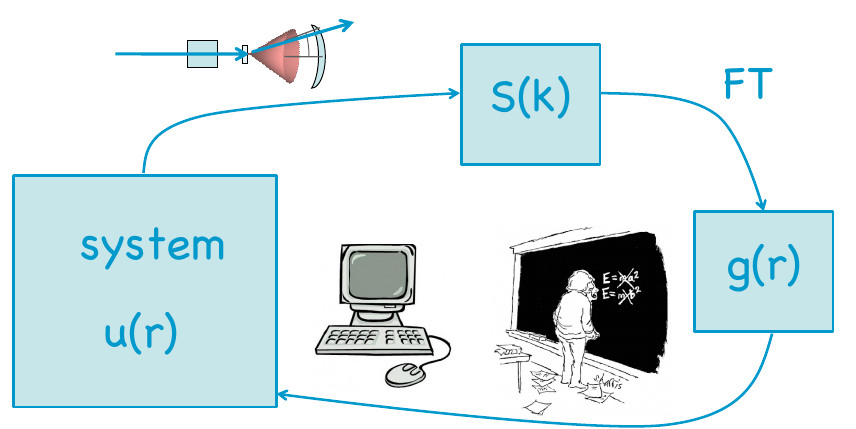
\includegraphics[width=0.5\textwidth]{figures/schema-iniziale-ur-gr.png}
	\caption{Passare dalla $g(r)$ alla $u(r)$.}
	\label{fig:ur-gr}
\end{figure}
\subsubsection{Teorie molticorpi.}
\label{subsubsec:Teorie molticorpi.}
La relazione tra $u(r)$ e $g(r)$ può essere studiata all'interno delle teorie di multicorpi e di calcolo numerico. Questo approccio ha un costo computazionale quasi nullo ma richiede spesso delle approssimazioni importanti per gestire l'interazione a molticorpi.
\subsubsection{Simulazioni al computer}
\label{subsubsec:Simulazioni al computer}
Possiamo simulare un set di particelle con un potenziale di interazione scelto dal programmatore $u(r)$, a questo punto abbiamo che $g(r)$ può essere estrapolata lanciando la simulazione e lasciandola andare per un tempo sufficientemente lungo.\\
Questo approccio è molto simile a fare un esperimento vero, l'artificialità è introdotta dal poter scegliere la $u(r)$. \\
L'unico limite di questo approccio è la potenza di calcolo del computer, inoltre per avere dei risultati fisici significativi è necessario poter accedere a dei dati veri di $g(r)$ altrimenti resta soltanto un giocattolo.
\subsection{Unicità della relazione tra $g(r)$ e $u(r)$.}
\label{subsec:Unicità della relazione tra $g(r)$ e $u(r)$.}
Abbiamo visto che la relazione tra la $S(q)$ e la $g(r)$ è unicamente determinata tramite una FT, si può dire lo stesso tra $g(r)$ e $u(r)$? Esiste una relazione che determina in modo biunivoco il legame tra la $u$ e la $g$?\\
Prendiamo un sistema di particelle in cui il potenziale agisce soltanto tra i primi vicini, in questo caso la $u(r)$ determina in modo univoco la $g(r)$. Potremmo dire anche il viceversa?\\
Ci chiediamo quindi se è vero che ad ogni funzione di distribuzione di coppia corrisponde un unico potenziale di coppia $u(r)$.\\
La risposta è si, sotto alcune ipotesi:
\begin{fact}[La relazione che lega $g(r)$ ad una singola $u(r)$ è unica e biunivoca.]{fact:La relazione che lega $g(r)$ ad una singola $u(r)$ è unica e biunivoca.}
	$g(r)$ e $u(r)$ sono biunivocamente legate se:
	\begin{itemize}
		\item Siamo all'equilibrio termodinamico.
		\item Siamo in un sistema in cui agiscono soltanto le forze a 2 particelle.
		\item I potenziali che differiscono di una costante corrispondono alla
			stessa $g(r)$.
	\end{itemize}
\end{fact}
Per la dimostrazione di questo teorema riporto una reinterpretazione (traduzione) dell'articolo di Henderson. L'autore considera un sistema di $N$ particelle identiche alla temperatura $T$ in un volume $V$, l'Hamiltoniana è data da:
\[
    H = \sum_{i}^{} \frac{p^2_i}{2M}+ \frac{1}{2}\sum_{i\neq j}^{} u(\v{r}_i-\v{r}_j) 
.\] 
Possiamo scrivere il potenziale interatomico mediante la funzione di distribuzione di coppia $n_2(\v{r},\v{r}')$ (la nostra $\rho_2$ moltiplicata per il numero medio di particelle) e trasformando la somma sulle posizioni $i$  e $j$  in integrale:
\[
    \left<\frac{1}{2}\sum_{i\neq j}^{} u(\v{r}_i-\v{r}_j)\right> = \frac{1}{2}\int \v{r}d\v{r}'u(\v{r}-\v{r'}) n_2(\v{r},\v{r}') 
.\] 
Se andiamo nel limite termodinamico allora la funzione di distribuzione di coppia diventa:
\[
    n_2 \to n^2g(r) 
.\] 
Dove $n$ è la densità media di particelle e la $g(r)$ è la funzione vista nella lezione scorsa (qui chiamata funzione di distribuzione radiale).
Il teorema di unicità segue da una disuguaglianza sulla energia libera di Halmotz: consideriamo due sistemi sotto condizioni di temperatura, densità e volume identici ma descritti da due Hamiltoniane diverse $H_1$ e $H_2$; sia nel caso classico che nel caso quantistico le corrispondenti energie libere sono legate dalla seguente disuguaglianza:
\[
    F_2\le F_1 + \left<H_2-H_1\right>_1 \label{eq:Halmotz-Badasss}
.\] 
Dove si media con la misura adatta ad $H_1$. La relazione sopra diventa una uguaglianza se $H_2-H_1$ è indipendente dagli impulsi e dalle coordinate.\\
Consideriamo quindi due sistemi identici in ogni aspetto eccetto il potenziale di coppia $u(r)$ e $u'(r)$, le corrispondenti funzioni di distribuzione di coppia sono $n_2$ e $n_2'$. \\
Il teorema di unicità che stiamo dimostrando afferma che se $n_2(\v{r},\v{r}') = n'_2(\v{r},\v{r}')$ per ogni $\v{r}$ e $\v{r}'$ allora i potenziali non possono differire per più di una costante.\\
Procediamo per assurdo negando l'ultima affermazione, in questo modo per ogni temperatura la condizione per avere una uguaglianza in equazione \ref{eq:Halmotz-Badasss} sarebbe violata; si avrà quindi:
\[
    F< F' + \left<H-H'\right>'=
    F'+\frac{1}{2}\int d\v{r}d\v{r}'\left[u(\v{r}-\v{r}') - u'(\v{r}-\v{r}') \right]n_2'(\v{r}\v{r}') 	
.\] 
Dove si usa la $n_2'$ perché fa parte della misura di media (della disuguaglianza). Possiamo dire che tale disuguaglianza debba valere anche per l'energia di Halmotz non primata, quindi:
\[
    F'< F + \left<H-H'\right>=
    F+\frac{1}{2}\int d\v{r}d\v{r}'\left[u(\v{r}-\v{r}') - u'(\v{r}-\v{r}') \right]n_2(\v{r}\v{r}') 	
.\] 
Se supponiamo che $n_2=n_2'$ per tutti gli $\v{r}$ e $\v{r}'$ allora abbiamo l'assurdo $0<0$.\\
Non è comunque garantita l'esistenza di una $u(r)$ per ogni $g(r)$, tuttavia esiste sempre una procedura numerica inversa quando le condizioni del Fatto \ref{fact:La relazione che lega $g(r)$ ad una singola $u(r)$ è unica e biunivoca.} sussistono.\\ 
\subsection{Energia interna di un fluido monoatomico classico con potenziale a 2 corpi.}
\label{subsec:Energia interna di un fluido monoatomico classico con potenziale a 2 corpi.}
Consideriamo un fluido monoatomico con un potenziale di interazione che agisce solo a due particelle:
\[
	U = \sum_{i<j}^{} u(r_{ij}) \quad \quad  r_{ij} = \left| \v{r}_i - \v{r}_j \right| 
.\] 
La media dell'energia potenziale totale del sistema si ottiene come:
\[\begin{aligned}
	\left<U \right> 
	=&
	\frac{1}{Z}\int d \v{r}_1\ldots d \v{r}_N 
	\sum_{i<j}^{} u(r_{ij})
	\exp\left( -\sum_{i<j}^{} u(r_{ij})/kT \right) =\\
	=&
	\frac{N\left( N-1 \right) }{2} 
	\int d \v{r}d \v{r}' u(\left|\v{r}-\v{r}'\right|)
	\left[ 
	\ffrac{
	\int d\v{r}_1\ldots d\v{r}_N
	\exp\left(-\sum_{i<j}^{} u(r_{ij})/kT\right) 
	\delta(\v{r}-\v{r}_1)\delta(\v{r}'-\v{r}_2)
	}{Z} \right] =\\
	=&
	\frac{N(N-1)}{2} \int d \v{r} d \v{r}' u(\left| \v{r}-\v{r}' \right|)
	g(\left| \v{r}-\v{r}' \right|)\rho ^2\frac{\left( N-2 \right)!}{N!} =\\
	=&
	\frac{1}{2} \rho ^2 V \int u(r)g(r)4\pi r^2 dr
.\end{aligned}\]
Nel primo passaggio abbiamo assunto che $u(r_{ij})$ sia lo stesso per tutte le particelle, quindi abbiamo esplicitato le $N(N-1) /2$ sommatorie lasciando il potenziale in dipendenza di sue singole particelle: $\v{r}_1$ e $\v{r}_2$. \\
Visto che ci è ancora comodo avere un integrale su tutte le particelle (che escluda la $u$ non in forma esponenziale) allora si trasformano i rimanenti $N-2$ integrali in $N$ integrali introducendo le due $\delta$. Procedendo in questo modo la quantità da parentesi è esattamente la $\overline{\rho}_2$.\\
La definizione di $\overline{\rho}_2$ è infatti:
\[
	\overline{\rho }_2(\v{r}_1,\v{r}_2) 
	= 
	\left< \sum_{i\neq j}^{} \delta(\v{r}_1 -\v{r}_i)\delta(\v{r}_2 - \v{r}_j) \right>
.\] 
Che nel formalismo gran canonico diventa proprio l'espressione tra parentesi quadre. Se poi ricordiamo che per i liquidi si ha anche che:
\[
	\overline{\rho }_2(\left| \v{r}_1 -\v{r}_2 \right| )
	=
	\rho ^2 g(\left| \v{r}_1 - \v{r}_2 \right| )
.\] 
Si ottiene il passaggio discusso.\\
In conclusione troviamo che l'energia potenziale può essere espressa in termini del potenziale di coppia stesso pesato sulla funzione di distribuzione di coppia. L'energia interna di un fluido monoatomico classico così descritto sarà:
\[
	E = \frac{3}{2}NkT 
	+
	\frac{N}{2}\rho \int u(r)g(r)4\pi r^2 dr
.\] 
Se il potenziale è indipendente dalla temperatura allora possiamo esprimere il calore specifico come:
\[
	C_V =
	\frac{3}{2}Nk 
	+
	\frac{N}{2}\rho \int u(r)\frac{\partial g(r)}{\partial T} 4\pi r^2 dr
.\] 
Passando invece dal teorema del Viriale per sistemi confinati:
\[
	2\left<K \right> = - \sum_{}^{} \v{F}_i\cdot\v{r}_i
.\] 
si ottiene una generalizzazione della leggi di stato per i gas perfetti in presenza di una interazione di coppia:
\[
	2 \frac{3}{2}NkT 
	=
	3PV
	+
	N \frac{\rho }{2}\int r \frac{\partial u(r)}{\partial r} g(r) dr
	\label{eq:virial-trick}
.\] 
Quindi anche:
\begin{defn}[Generalizzazione della equazione di stato]{def:Generalizzazione della equazione di stato}
	\[
	P 
	=
	\rho kT - \frac{\rho ^2}{6}\int r \frac{\partial u(r)}{\partial r} g(r) dr
	.\]
\end{defn}
Notiamo che finche non si trova una relazione diretta tra $u(r)$ e $g(r)$ non è possibile risolvere con la correzione tale equazione.
\subsubsection{Digressione sulla derivazione della equazione di stato a partire dal Viriale.}
\label{subsubsec:Digressione sulla derivazione della equazione di stato a partire dal Viriale.}
Nella equazione \ref{eq:virial-trick} abbiamo che il secondo termine deriva dalle interazioni tra le particelle interne al gas mentre il termine $3PV$ dovrebbe essere un termine di pressione di bordo. Per dimostrarlo mettiamoci all'interno di una sfera avente raggio $R$ come in Figura \ref{fig:sfera-per-dimostrare-la-relazione-di-gas-perfetto} e trascuriamo l'interazione $u(r)$.
\begin{figure}[ht]
    \centering
    \incfig{sfera-per-dimostrare-la-relazione-di-gas-perfetto}
    \caption{Sfera per dimostrare la relazione di gas perfetto}
    \label{fig:sfera-per-dimostrare-la-relazione-di-gas-perfetto}
\end{figure}
Per il calcolo di $\v{F}\cdot\v{r}$ conviene passare dalla sommatoria ad un integrale in $d \v{r}$:
\[
	\sum_{i}^{} \v{F}_i\cdot\v{r}_{i} \to 
	\int\v{r}\cdot\v{F} \delta(r-R)dr
.\] 
Dove abbiamo introdotto il fatto che la forza sta solo sulla superficie tramite una $\delta(\v{r}-\v{R})$ \footnote{Ricordiamoci che la $\delta$ porta le dimensioni di un inverso di una lunghezza, quindi il calcolo è dimensionato.}.
Possiamo calcolare la forza come 
\[
	\v{F} = \int P d \v{s}
.\] 
Dove $d \v{s} \propto - \hat{r}$.
Inserendo anche questa si ha che:
\[\begin{aligned}
	\int dr\delta(r-R)  \v{F}\cdot\v{r}
	=&
	\int\int dr\delta(r-R)P \v{r}\cdot  d \v{s} =\\
	=&
	-\int d V Pr \delta(r-R) =\\
	=&
	-4\pi\int r^3 \delta(r-R)P dr =\\
	=&
	-3PV
.\end{aligned}\]
In conclusione si ottiene quanto atteso (visto che nel teorema c'è un segno negativo).
\subsubsection{Digressione su potenziali del tipo $u(r) \propto r^n$.}
\label{subsubsec:Digressione su potenziali polinomiali.}
Per potenziali di questo tipo si ha che il teorema del Viriale assume la forma:
\[
	2\left<K \right> = n\left< U \right>
.\] 
Non saprei\ldots\\
\subsubsection{Digressione: legge di stato nel caso di gas quantistici.}
\label{subsubsec:Digressione: legge di stato nel caso di gas quantistici.}
Nel caso di gas quantistico abbiamo una correzione quantistica alla legge di stato del seguente tipo:
\[
	\frac{P}{\rho kT}
	=
	1 \pm \frac{\rho \lambda^3(T)}{4\sqrt{2} \left( 2s + 1 \right) }
.\] 
Dove il segno positivo è per i fermioni mentre quello negativo per i bosoni (come abbiamo già visto). Nella formula $\lambda$ è la lunghezza d'onda di De Broglie:
\[
	\lambda=\sqrt{\frac{h^2}{3mkT}} 
.\] 
\subsection{Ricerca di una relazione analitica tra $u(r)$ e $g(r)$.}
\label{subsec:Ricerca di una relazione analitica tra $u(r)$ e $g(r)$.}
Tramite Simulazioni al computer è sempre possibile ottenere l'espressione per $S(q)$ e $g(r)$ fissata una $u(r)$, basta creare il sistema di particelle, farlo termalizzare (andare all'equilibrio) e poi valutare numericamente le quantità cercate. \\
Il vantaggio del metodo precedente è che possiamo decidere un potenziale a piacere per il nostro conto, lo svantaggio è la potenza di calcolo richiesta per simulare un sistema che assomigli a qualcosa di reale e il computer si porta dietro una incertezza numerica.\\
Se potessimo ottenere la relazione analitica tra la funzione di correlazione di coppia e il potenziale tra due particelle avremo idealmente risolto il nostro sistema. Tuttavia vedremo che questo è un problema non risolvibile analiticamente.\\
Vediamo come si procede analiticamente a grandi linee per arrivare ad un risultato. Per far questo ci è utile sfruttare la definizione di media di $\overline{\rho }_2$ nell'Ensemble gran canonico:
\[
	\overline{\rho }_2(\v{r}_1,\v{r}_2) =
	\sum_{N=2}^{} \frac{1}{Z_N N!}\int \prod_{I,J}^{} d \v{r}_I d \v{P}_J 
	\exp\left(
	-\frac{ K(\left\{ \v{P}_J \right\}) + U(\left\{ \v{r}_I \right\} ) }{kT} \right)
	\sum_{i\neq j}^{} \delta(\v{r}_1-\v{r}_i)\delta(\v{r}_2-\v{r}_j)
.\] 
Nel caso di fluidi questa espressione si semplifica sensibilmente diventando la seguente formula:
\[
	\rho ^2g(\left| \v{r}_1-\v{r}_2 \right|)
	=
	\frac{1}{\Upxi}
	\sum_{N=2}^{} \frac{z^{N}}{(N-2)!}
	\int e^{-U(\v{r}_1,\ldots,\v{r}_N)/kT} d \v{r}_3\ldots d \v{r}_N
	\label{eq:brutta-eq}
.\] 
In cui ricordiamo la Fugacità già incontrata in precedenza:
\[
	z = \left( \frac{mkT}{2\pi\hbar ^2} \right) ^{3/2}e^{\mu /kT}
.\] 
E la funzione di partizione gran canonica $\Upxi$:
\[
	\Upxi = 
	\sum_{N=0}^{} \frac{z^{N}}{N!}\int e^{-U(\v{r}_1,\ldots,\v{r}_N)/kT}
	d \v{r}_1\ldots d \v{r}_N
.\] 
Abbiamo quindi una complicata equazione per la densità di massa a due corpi, infatti a peggiorare ancora la situazione all'interno dell'esponenziale abbiamo pure:
\[\begin{aligned}
	U(\v{r}_1,\ldots,\v{r}_N) =&
	\sum_{i>j}^{} u(\left| \v{r}_i - \v{r}_j \right| )=\\
	=&
	u(\left| \v{r}_1-\v{r}_2 \right| ) 
	+
	\sum_{i=3}^{} u(\left| \v{r}_1-\v{r}_i \right| ) 
	+
	\left( \text{Term. indip. da } \v{r}_1 \right) 
.\end{aligned}\]
Aver scritto il potenziale in questo modo ci aiuta perché se adesso prendiamo il gradiente della equazione \ref{eq:brutta-eq} rispetto a $\v{r}_1$ otteniamo:
\[\begin{aligned}
	\rho ^2\nabla_{\v{r}_1}g(\left| \v{r}_1-\v{r}_2 \right| ) =
	- \frac{1}{kT} \nabla_{\v{r}_1}u(\left| \v{r}_1-\v{r}_2 \right|)
	\underbrace{
	\frac{1}{\Upxi}\sum_{N=2}^{} \frac{z^N}{(N-2)!}
	\int e^{- U(\v{r}_1,\ldots,\v{r}_N)/kT}d \v{r}_3\ldots d \v{r}_N 
	}_{=\rho ^2 g(r)}
	+ \\
	- \frac{1}{kT} \frac{1}{\Upxi} \sum_{N=2}^{} \frac{z^N}{(N-2)!}
	\int d\v{r}_3 \ldots d \v{r}_N e^{-U(\v{r}_1,\ldots,d \v{r}_N)/kT}
	\sum_{i=3}^{} \nabla_{\v{r}_1}u(\left| \v{r}_1 - \v{r}_i \right| )
	\label{eq:nabla-g}
.\end{aligned}\]
Che a prima vista non sembra molto bella, tuttavia nasconde dei piccoli segreti. Infatti facendo una cosa analoga a quanto fatto per il calcolo della $\left<U \right>$ ad inizio lezione possiamo anche qui trasformare una sommatoria in un prodotto di integrali utilizzando 3 $\delta$. \\
In questo modo è possibile definire una funzione di distribuzione al terzo ordine:
\[
	\left<\rho _3(\v{r},\v{r}',\v{r}'') \right> 
	=
	\left< 
	\sum_{i,j,k}^{} 
	\delta(\v{r}_i-\v{r})\delta(\v{r}_j-\v{r}')\delta(\v{r}_k-\v{r}'')
	\right>
.\] 
Che nel caso di fluidi diventerà:
\[\begin{aligned}
	\left<\rho _3(\v{r},\v{r}',\v{r}'') \right> 
	=&
	\rho ^3 g_3(\v{r},\v{r}',\v{r}'') =\\
	=&
	\frac{1}{\Upxi}\sum_{N=3}^{} 
	\frac{z^N}{(N-3)!}\int e^{-U(\v{r}_1,\ldots,\v{r}_N)/kT} d \v{r}_4\ldots d \v{r}_N
.\end{aligned}\]
Inserendo questa nella equazione \ref{eq:nabla-g} si ottiene:
\[
	\nabla_{\v{r}_1} g(\left| \v{r}_1-\v{r}_2 \right| ) 
	=
	- \frac{g(\left| \v{r}_1 -\v{r}_2\right| )}{kT}  
	\nabla_{\v{r}_1}u(\left| \v{r}_1-\v{r}_2 \right|) 
	-
	\frac{\rho }{kT} \int d \v{r}_3\nabla_{\v{r}_1}u(\left| \v{r}_1-\v{r}_3 \right|)
	g_3(\v{r}_1,\v{r}_2,\v{r}_3)
	\label{eq:non-approx-g}
.\] 
Notiamo che l'integrale che coinvolge la $g_3$ è un integrale di convoluzione. È proprio questo termine il problema dell'approccio analitico: senza questo la relazione tra $g$ ed $u$ sarebbe semplice e anche invertibile.\\
L a $g_3$ può essere scritta anche in funzione della distanza tra i tre  $\v{r}_i$,in questo modo mi bastano due distanze per poterla descrivere, la terza dipenderà dalle altre due. Definiamo allora:
\[\begin{aligned}
	& r = \left| \v{r}_1-\v{r}_2 \right| \\
	&r' = \left| \v{r}_1-\v{r}_3 \right| 
.\end{aligned}\]
In modo tale da scrivere in modo ancora più compatto l'equazione sopra sfruttando anche l'isotropia del fluido:
\begin{fact}[Collegamento tra $g(r)$ e $u(r)$ mediato dalla $g_3(r,r')$.]{fact:Collegamento tra $g(r)$ e $u(r)$ mediato dalla $g_3(r,r')$.}
	In un fluido il collegamento tra il potenziale a due particelle e la funzione 
	di correlazione di coppia è mediato dalla $g_3(r,r')$ tramite la seguente:
	\[
	\nabla g(r) = -\frac{g(r)}{kT} \nabla u(r)
	- \frac{\rho }{kT}\int d \v{r}'\nabla u(r')g_3(r,r')
	.\] 
\end{fact}
Andando avanti con il conto di si rende presto conto che non è ancora finita, infatti per calcolare la $g_i$ serve la $g_{i+i}$, si innesca una catena che non si ferma. L'unico modo per rendere risolvibile questa equazione è di chiudere la catena delle $g_i$ inventandosi una approssimazione per la $g_3$ in funzione di $g(r)$ e $u(r)$. Procediamo allora proprio in questo modo:
\[
	\frac{\nabla g(r)}{g(r)}
	=
	\nabla\left[ \ln(g(r)) \right] 
	=
	- \nabla  \frac{u(r)}{kT} 
	-
	\frac{\rho }{kT g(r)} \int d \v{r}' \nabla u(r)g_3(r,r')
.\] 
Possiamo quindi procedere assumendo che la $g_3$ sia trascurabile rispetto alla $g$, in questo modo l'equazione diventa:
\[
	\nabla\left[ \ln(g(r))+\frac{u(r)}{kT} \right] = 0
.\] 
In questo modo otteniamo una legge alla Boltzmann tra $g$ ed $u$:
\[\begin{aligned}
	& g(r) = e^{-\frac{u(r)}{kT}}\\
	& u(r) = - kT\ln (g(r))
.\end{aligned}\]
Notiamo che questa legge sarebbe rigorosamente vero se avessi soltanto due particelle nel sistema, possiamo assumere che sia vero anche nel caso di gas molto rarefatti.\\
È comunque utile definire un $w(r)$ al posto di $u(r)$ nell'esponenziale, questo termine a differenza di $u$ tiene conto dell'effetto di $g_3$ nella equazione ed è chiamato potenziale di forza media (PMF).
\[\begin{aligned}
	& g(r) = e^{-\frac{w(r)}{kT}}\\
	& w(r) = - kT\ln (g(r))
.\end{aligned}\]
Passare dall'una all'altra formula significa fare l'inversione di Boltzmann.
\subsection{Potenziali $u(r)$ e $w(r)$ in un fluido di Lennard Jones.}
\label{subsec:Potenziali $u(r)$ e $w(r)$ in un fluido di Lennard Jones.}
Abbiamo visto che per un fluido di Lennard Jones Abbiamo una $g(r)$ della forma di \ref{fig:figures-slide-tesi-png}. Effettuando l'inversione di Boltzmann su tale andamento di ottiene:
\begin{figure}[H]
	\centering
	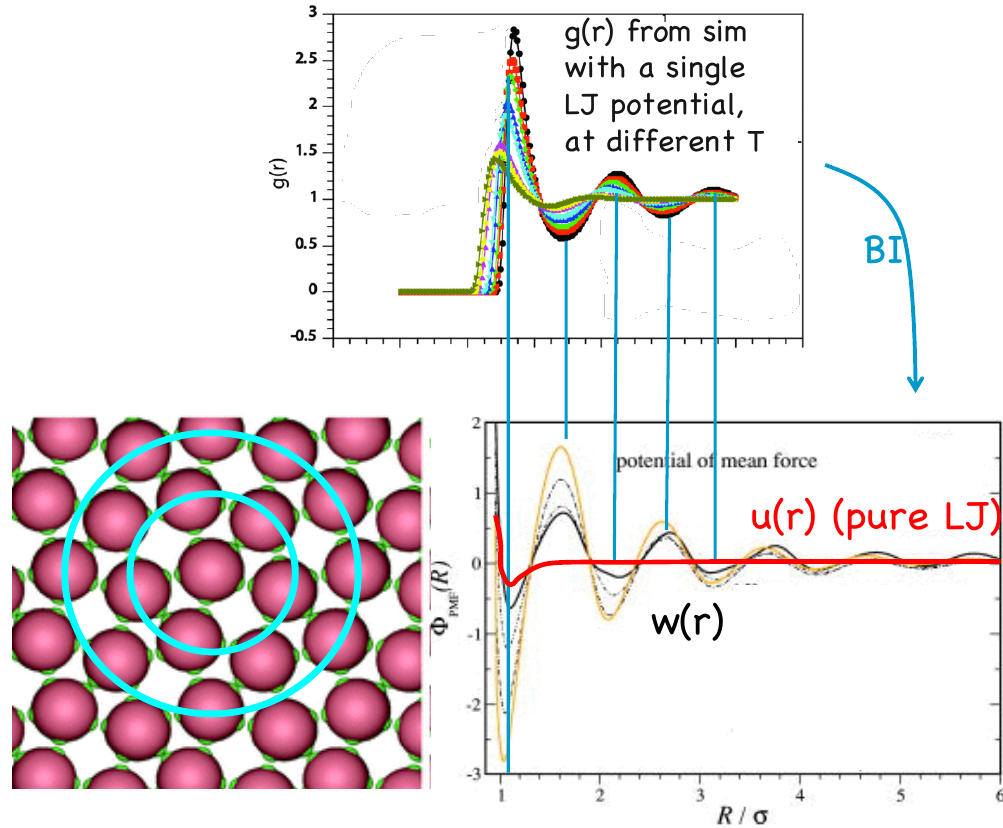
\includegraphics[width=0.6\textwidth]{figures/wug-andamenti.png}
	\caption{figures/wug-andamenti.png}
	\label{fig:figures-wug-andamenti-png}
\end{figure}
\noindent
Notiamo che l'inversione di Boltzmann converte i massimi di $g(r)$ in minimi di $u(r)$.\\
Inoltre è evidente la differenza tra il potenziale $u(r)$ e $w(r)$, quest'ultimo infatti è molto più strutturato di $u$, l'unica cosa da tenere bene in considerazione è il fatto che il primo minimo è lo stesso per tutti e due i potenziali. \\
\subsection{Chiusura di Born-Green.}
\label{subsec:Chiusura di Borhn Green.}
Considerando l'espressione non approssimata (eq. \ref{eq:non-approx-g}) possiamo provare a vedere se esistono altri modi di chiuderla senza perdere troppe informazioni. Un metodo è quello di Born-Green, questo consiste nel considerare la $g_3$ come catena di funzioni di correlazione di coppia:
\[
	g_3(\v{r}_1,\v{r}_2,\v{r}_3)
	=
	g(\left|\v{r}_1-\v{r}_2\right|) 
	g(\left|\v{r}_2-\v{r}_3\right|) 
	g(\left|\v{r}_1-\v{r}_3\right|)
.\]
Questa approssimazione è anche detta approssimazione di sovrapposizione.\\
Per procedere con i conti di Born e Green è necessario richiamare alcune quantità e definirne altre in modo da poter riscrivere l'equazione da risolvere. Partiamo dalle 3 variabili:
\[\begin{aligned}
	&r_2-r_1 = r\\
	&r_3-r_2 = r' \\
	&r_3-r_1 = r'-r
.\end{aligned}\]
Riscriviamo ed introduciamo adesso:
\[\begin{aligned}
	&
	\overbrace{
	\ln(g(r))}^{-\frac{w(r)}{kT}} + \frac{u(r)}{kT} 
	=
	\rho \int E(\left| \v{r}-\v{r}' \right|)h(r')d \v{r}'\\
	&h(r) = g(r)-1\\
	&E(x) = \frac{1}{kT}\int_{x}^{\infty}g(x')\frac{\mbox{d} u}{\mbox{d} x} (x')dx' 
	\label{eq:B-G-approx}
.\end{aligned}\]
La funzione di supporto $E(x)$ ha la proprietà 
\[\begin{aligned}
	&E(x) = -\frac{u(x)}{kT} \quad \text{ Se } \quad g \sim 1\\
	&E(x) = 0 \quad \quad\text{ Per gas ideali}\\
	&FT\left[ E \right] (k=0) = \overline{E}(0) = 2\left[ 1-\frac{P}{\rho kT} \right] 
.\end{aligned}\]
In questo modo la relazione tra $u(r)$ e $g(r)$ è chiusa e può essere risolta (almeno numericamente).
\subsection{Funzione di correlazione diretta.}
\label{subsec:Funzione di correlazione diretta.}
Per continuare la trattazione conviene introdurre anche una funzione di correlazione diretta $c(r)$ come:
\begin{defn}[Funzione di correlazione diretta]{def:Funzione di correlazione diretta}
	Si dice Funzione di correlazione diretta $c(r)$ la funzione per la quale vale la   
	seguente relazione:
	\[
		h(r) = 
		c(r) 
		+
		\rho \int d \v{r}'h(\v{r'})c(\left| \v{r}-\v{r}' \right| )
	.\] 
\end{defn}
Questa funzione è quindi collegata alla Hole function da un prodotto di convoluzione, vorrà dire che in trasformata si potranno ottenere delle relazioni più semplici del tipo:
\[\begin{aligned}
	&\overline{h}(k) = \overline{c}(k) + \overline{h}(k) \overline{c}(k) 
	\implies \overline{h}(k) = \frac{\overline{c}(k)}{1-\overline{c}(k)}\\
	&\overline{c}(k) = \frac{\overline{h}(k)}{1 + \overline{h}(k)}=
	\frac{S(k)-1}{S(k)} = 1 - \frac{1}{S(k)}
.\end{aligned}\]
La funzione $c(r)$ ha anche la proprietà:
\[
	h(r\to \infty) = 0
.\]
Inoltre si può ricavare che:
\[
	\int h(r)d \v{r} = S(0)-1 = \rho kT K_T -1 = 
	\begin{cases}
		&0 \quad \text{ Per gas perfetti}\\
		&-1 \quad \text{ Per fluidi in comprimibili}
	\end{cases}
\] 
\[
	\int c(r)d \v{r} = \overline{c}(0)= 1- \frac{1}{\rho kTK_T}
.\] 
Abbiamo che $c,h,g$ ed $S$ contengono tutte le medesime informazioni, se sperimentalmente ne troviamo una possiamo ricavare da questa tutte le altre.\\
Per concludere la carrellata mettiamo una tabella di cose utili da ricordare:
\begin{figure}[H]
	\centering
	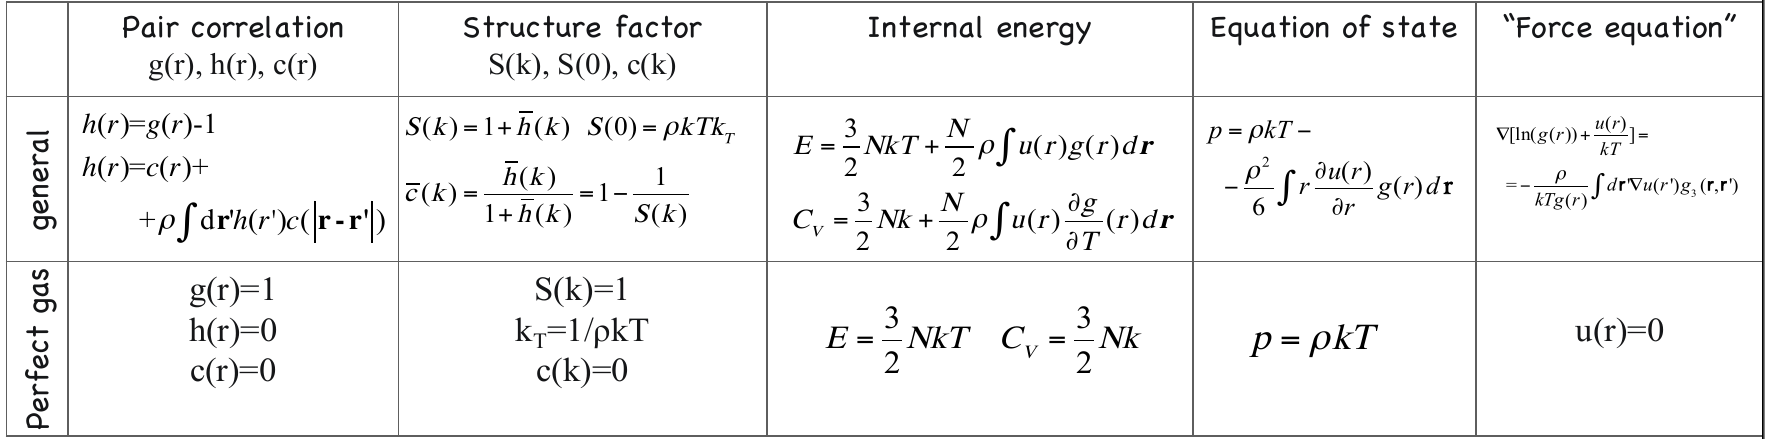
\includegraphics[width=0.9\textwidth]{figures/riassuntone-lez3-liquidi.png}
	\caption{Riassunto delle formule salienti affrontate fino ad ora.}
	\label{fig:figures-riassuntone-lez3-liquidi-png}
\end{figure}
\subsection{Modelli a sfere}
Se volessimo studiare un gas perfetto allora abbiamo già tutto quello che ci serve \footnote{Ricordiamo che in questo caso si ha una $S(q)$ piatta e da questa derivano tutte le semplificazioni.}. Il modello più facile che possiamo incontrare dopo il gas perfetto è quello delle sfere dure:
\begin{figure}[H]
    \centering
    \incfig{sfere-dure-u}
    \caption{Modello di potenziale a "sfere dure".}
    \label{fig:sfere-dure-u}
\end{figure}
\noindent
In questo modello il potenziale è nullo fino a che le due sfere non si toccano, a quel punto diventa improvvisamente $\infty$.\\
Tuttavia avere una netta divergenza porta problemi sia dal punto di vista numerico \footnote{Un potenziale così Hardcore mi da sempre problemi nel calcolo di integrali, nelle simulazioni reali si usano potenziali analitici più soft (nelle simulazioni di dinamica molecolare standard)} sia dal punto di vista analitico dove alcuni integrali con questi oggetti potrebbero portare problemi. \\
Per ovviare a questo problema si costruisce il modello a sfere soffici:
\begin{figure}[H]
    \centering
    \incfig{sfere-soffici-u}
    \caption{Modello di potenziale a "sfere soffici".}
    \label{fig:sfere-soffici-u}
\end{figure}
\noindent
Questo modello può essere considerato un buon modello per i colloidi.\\
In conclusione abbiamo il modello di Lennard Jones che introduce un termine $\mathcal{E}$ di attrazione tra le sfere, il potenziale prende così la forma:
\begin{figure}[H]
    \centering
    \incfig{sfere-lennard-jones}
    \caption{Modello di Lennard Jones.}
    \label{fig:sfere-lennard-jones}
\end{figure}
\noindent
\subsection{Modello a sfere dure.}
\label{subsec:Modello a sfere dure.}
Possiamo partire per questa analisi dalla equazione di stato per il sistema:
\[
	\frac{P}{\rho kT} 
	=
	1-\frac{\rho }{6}\int r \frac{\partial u(r)/kT}{\partial r} g(r) d \v{r}
.\] 
Mentre l'equazione di forza è:
\[
	\ln(g(r))+\frac{u(r)}{kT}
	=
	\rho \int d \v{r}'\left( g(r')-1 \right) 
	\int_{r-r'}^{\infty} g(x)\frac{\partial u(x)/kT}{\partial x} dx
.\] 
Notiamo che $u(r)$ dipende soltanto dal parametro $\sigma$ (il diametro della sfera), mentre l'equazione di forza dipende in $u$ soltanto tramite la combinazione $u(r)/kT$. Per come è definito il potenziale si ha che $C\cdot u(r) = u(r)$, questo implica che la $g(r)$ è indipendente dalla temperatura.\\
Visto che la scala di lunghezze del sistema è $\sigma$ possiamo riscrivere tutto in funzione di $x = r/\sigma$ e della densità espressa tramite la frazione di impacchettamento:
\[
	\eta = \rho \frac{4}{3}\pi R^3 = \pi\rho \frac{\sigma^3}{6} = \rho \nu
.\] 
In cui abbiamo usato il fatto che $R=\sigma /2$. Notiamo che non si avrà mai $\eta=1$, infatti per delle sfere FCC (le più compatte) raggiungiamo $\eta \approx 0.74$: resta sempre spazio tra gli atomi.\\
Inoltre $g(r)$ è identicamente nulla per $r<\sigma$ ed $u$ è nulla per $r>\sigma$ ma ovviamente $u$ e la sua derivata divergono a $r=\sigma$. Queste ultime considerazioni rendono difficile il calcolo degli integrali nelle equazioni.\\
Proviamo adesso a risolvere l'equazione di stato, essendo le sfere dure "ideali" potremmo assumere che queste si comportino come tali fino a che non entrino a contatto, quindi ciò che cambia dal modello di gas ideale è il volume a disposizione: se prima era $V$ adesso è $V-b$ dove $b$ è il co-volume. \\
Tale co-volume è esattamente 8 volte il volume di una singola sfera, lo possiamo capire dalla seguente figura:
\begin{figure}[H]
	\centering
	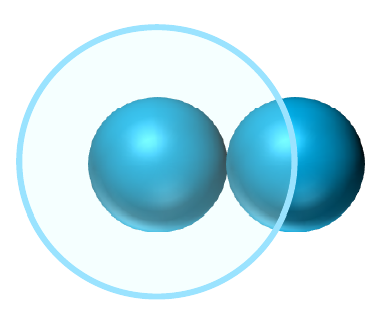
\includegraphics[width=0.2\textwidth]{figures/coovolume.png}
	\caption{Calcolo del co-volume per sfere dure.}
	\label{fig:figures-coovolume-png}
\end{figure}
\noindent
Dalla figura è evidente che la sfera non cerchiata non potrà spostarsi per tutto il volume in semi trasparenza attorno alla sfera di sinistra, tale sfera semitrasparente ha raggio doppio rispetto alle due sfere, quindi ha volume 8 volte maggiore. Questo risultato va diviso per due perché coinvolge due sfere. Ne risulta che se il volume di una sfera è $v$ allora il volume a disposizione è $V-4v$.\\
Risolvendo quindi l'integrale nella equazione di stato arriviamo alla seguente equazione\ldots
\[
	\frac{P}{\rho kT} = \frac{1}{1-4\eta}
.\] 
Questa è tanto più vera quanto più possiamo trascurare l'interazione a 3 particelle, ovvero per basse densità (bassi $\eta$). Il risultato di questa soluzione è il seguente:
\begin{figure}[H]
	\centering
	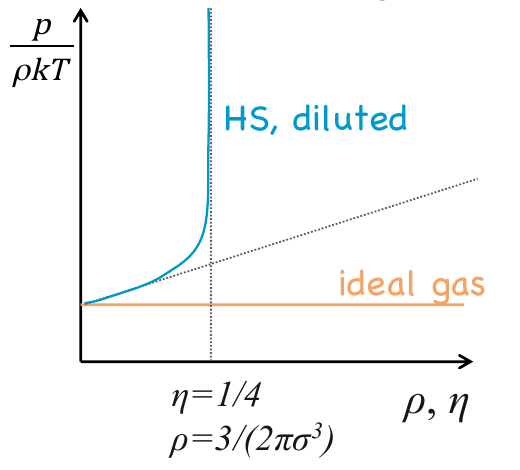
\includegraphics[width=0.3\textwidth]{figures/HS-diluited1.png}
	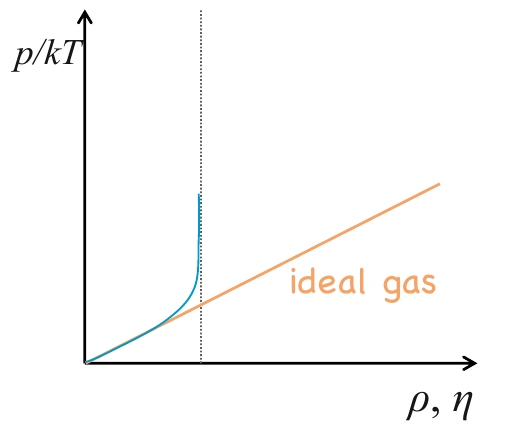
\includegraphics[width=0.3\textwidth]{figures/HS-diluited2.png}
	\caption{Modello a sfere dure a confronto con gas perfetto (i due grafici mostrano la stessa cosa).}
	\label{fig:figures-HS-diluited1-png}
\end{figure}
\noindent
Siamo portati a credere che la pressione diverga quando $\eta=1/4$, tuttavia si ha che l'approssimazione fallisce prima. Sappiamo infatti che il fattore di impacchettamento massimo è oltre $\eta = 0.25$, quindi deve essere possibile costruire un grafico fino a tale valore senza divergenze. Per questo motivo tale asintoto è fittizio, è un sintomo del fallimento della approssimazione di interazione a due sole particelle.\\
Vediamo come si trasformano invece la $g(r)$ e la $S(q)$:
\begin{figure}[H]
	\centering
	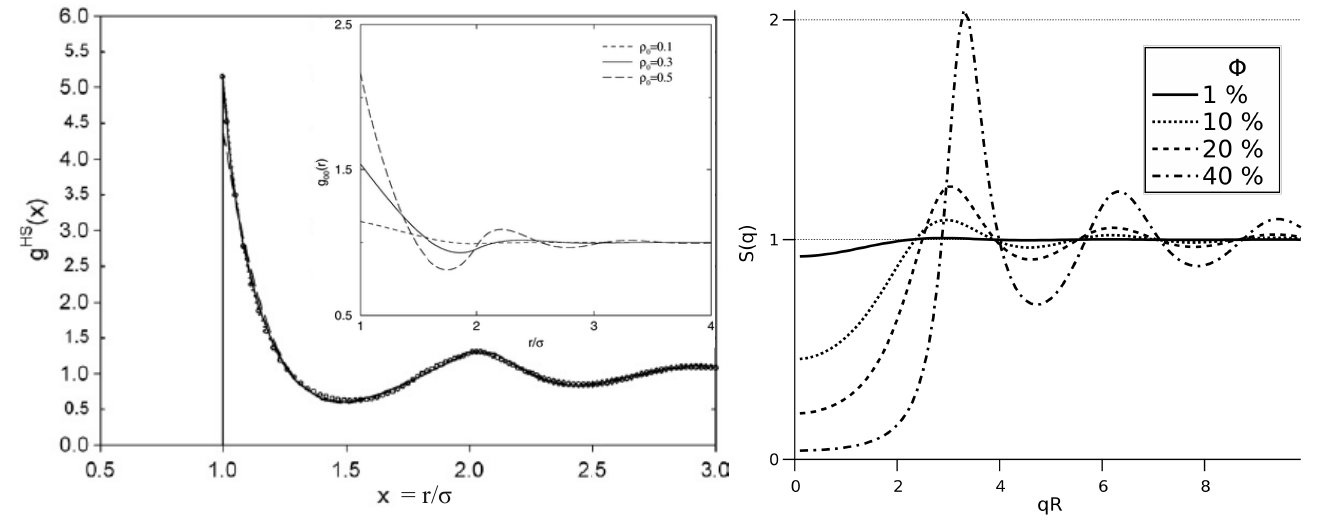
\includegraphics[width=0.6\textwidth]{figures/gr-sfera-dura.png}
	\caption{Andamento della $g(r)$ e della $S(q)$ per il modello a sfera dura.}
	\label{fig:figures-gr-sfera-dura-png}
\end{figure}
\noindent
Possiamo notare la discontinuità di $g(r)$ in $r/\sigma=1$, inoltre a basse densità entrambe le funzioni tendono ad 1. \\
Inoltre notiamo che la $g(r)$ e nulla per $x<1$ ma non è unitaria per $x>1$: la correlazione tra gli atomi è presente anche quando l'interazione è pressoché nulla (perché comunque si potrà avere contatto).\\
Quando le concentrazioni diventano grandi è necessario capire se il cristallo che si forma preferirà rimanere disordinato o sistemarsi in pacchetti. Ricordiamo intanto che il massimo fattore di impacchettamento ottenibile da delle sfere rigide è:
\[\begin{aligned}
	&\eta = \frac{\pi\sqrt{2} }{6} \approx 0.74\\
	&\rho = \frac{\sqrt{2}}{\sigma^3}
.\end{aligned}\]
In prossimità della densità critica del cristallo la compressibilità si annulla, quindi la pressione deve divergere essendo il sistema impossibile da comprimere. Quest'ultima affermazione ci fa capire che il sistema tenderà a sistemarsi in modo ordinato e che il grafico di $P/\rho kT$ divergerà dopo una fase ancora ignota.
\begin{figure}[H]
	\centering
	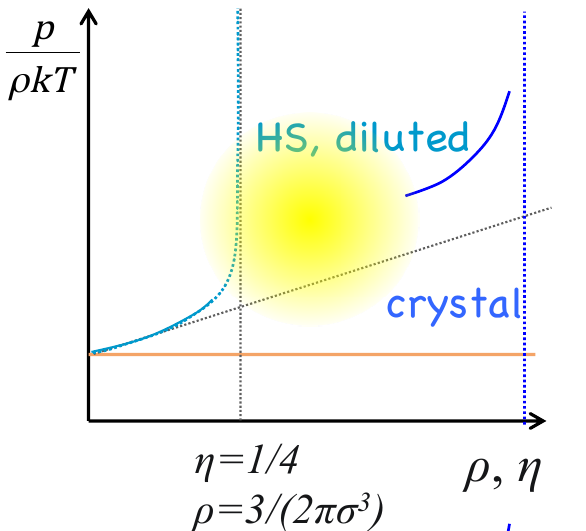
\includegraphics[width=0.4\textwidth]{figures/formato-cristallo-sfere-rigide.png}
	\caption{\scriptsize Zona in cui il cristallo è ormai formato, resta solo da capire cosa avviene nella zona centrale.}
	\label{fig:figures-formato-cristallo-sfere-rigide-png}
\end{figure}
\noindent
Per descrivere cosa avviene nella zona centrale è necessario utilizzare delle approssimazioni migliori alle due equazioni (stato e delle forze).
\subsection{Approssimazione di Abe.}
Un altro modo per risolvere in maniera analitica il problema alle Hard Sphere è l'approssimazione di Abe o Hypernetted Chain. \\
Riprendiamo le due equazioni:
\[\begin{aligned}
	&\text{Eq. stato:} \quad\frac{P}{\rho kT} 
	=
	1-\frac{\rho }{6}\int r \frac{\partial u(r)/kT}{\partial r} g(r) d \v{r}\\
	&\text{Eq. forze:}\quad\ln(g(r))+\frac{u(r)}{kT}
	=
	\rho \int d \v{r}'\left( g(r')-1 \right) 
	\int_{r-r'}^{\infty} g(x)\frac{\partial u(x)/kT}{\partial x} dx
.\end{aligned}\]
Consideriamo inoltre il potenziale di forza media $w(r)$:
\[
	w(r)=-kT\ln(g(r))
.\] 
Se sostituiamo questo integrale nella equazione di forza (la seconda sopra) si ottiene che:
\[
	\ln(g(r)) + \frac{u(r)}{kT} 
	=
	\rho \int d \v{r}'h(r')
	\left[\int_{r-r'}^{\infty} g(x)
	\frac{\partial \left[ \left( u-w \right) \right] /kT}{\partial x}dx 
	-
	\int_{r-r'}^{\infty} \frac{\partial g(x)}{\partial x} dx 
	\right] 
.\]
\paragraph{L'approssimazione}
L'approssimazione di Abe consiste nel porre all'interno dell'integrale contenente la derivata di $u-w$ il termine $g(r)\sim 1$. In questo modo l'equazione si semplifica nel seguente modo:
\[
	\ln(g(r)) + \frac{u(r)}{kT} 
	=
	\rho \int d\v{r}'h(r')\left[ \frac{w(r-r')-u(r-r')}{kT} + h(r-r') \right] 
.\] 
Infatti è stato sufficiente assumere che per $r\to \infty$ la differenza tra i due potenziali si annulli e che la $g(r)\to 1$ con $r\to \infty$.
\paragraph{Applicazioni fisiche della approssimazione di Abe}
L'approssimazione di Abe si può applicare a sistemi nei quali è possibile separare una interazione a corto range ed una a lungo range, questa risulta quindi molto buona per i potenziali di contatto mentre risulta pessima per i potenziali come Coulomb.
\paragraph{Legame della approssimazione con $c(r)$}
In maniera più pratica l'approssimazione di Abe può essere scritta ridefinendo la $c(r)$:
 \[\begin{aligned}
	 c(r) 
	 =&
	 \frac{w(r)-u(r)}{kT}+h(r)\\
	 =&
	 - \left[ \ln(g(r)) + \frac{u(r)}{kT} \right] + h(r)
	 \label{eq:1}
.\end{aligned}\]
In cui l'approssimazione si usa nel secondo passaggio.\\
In questo modo Abe è l'equivalente di porre $E(r)=c(r)$ nella equazione di stato:
\[
	\ln(g(r)) + \frac{u(r)}{kT} = \rho \int d\v{r}' h(r')c(r-r')
	\label{eq:2}
.\] 
Visto che si ha l'equazione \ref{eq:1} vale che, nel limite di grandi distanze rispetto a  $\sigma$ deve valere che:
\[\begin{aligned}
	&c(r) \approx -\frac{u(r)}{kT}\\
	&h(r) \approx -\frac{w(r)}{kT}
.\end{aligned}\]
Questo perché $\ln (g(r) ) \to 0$ e $h(r)\to 0$.\\
Dalla prima deriva il fatto che la funzione $c(r)$ si chiama funzione di correlazione diretta \footnote{Si vede infatti il collegamento diretto con il potenziale "nudo" di interazione} mentre dalla seconda il fatto che $h(r)$ si chiama funzione di correlazione totale.\\
Ricordiamo allora che $w(r)$ ed $h(r)$ contengono l'informazione della correlazione a molti corpi mentre $c(r)$ e $u(r)$ sono direttamente collegate al potenziale di interazione interatomico.\\
Il problema con i potenziali Hard core come quello a sfere rigide è il loro oscillare molto rapidamente nella regione di core.
Per trattare in maniera corretta tale regione si usa un'altra chiusura detta di Percus Yevick.
\subsection{Chiusura di Percus Yevick.}
Questa chiusura regolarizza la funzione $c(r)$ in vicinanza del core, infatti per le sfere dure abbiamo il problema che $u(r) \to \infty$ con $r\to \sigma$.
\begin{fact}[Apprrossimazione di Percus Yevick]{fact:Apprrossimazione di Percus Y}
	\[
		c(r) 
		\stackrel{\text{def}}{=} 
		-\frac{U_\text{eff}(r)}{kT}
		=
		g(r)\left[ 1-e^{u(r)/kT} \right] 
		=
		e^{-w(r)/kT}-e^{-\left[ w(r)-u(r) \right]/kT}
	.\] 
\end{fact}
Lo scopo di questa approssimazione è dare una espressione analitica per la $c(r)$ che sia nulla per $r>\sigma$ e polinomiale per $r<\sigma$. Inoltre la PY ci da anche una espressione esplicita per l'equazione di stato.
\paragraph{Utilità fisica}
Questo metodo risulta efficace quando siamo in situazioni di densità molto maggiori rispetto alla equazione di gas diluito, quindi funziona dove Abe fallisce. Infatti il metodo di Abe consiste nel mettere $g(r)\sim 1$ in un integrale contenente la differenza tra i potenziali, quindi in un certo senso assume il gas molto diluito, questa chiusura possiamo affermare che "mette una pezza" ai problemi di Abe.
\paragraph{Risultato della approssimazione PY}
Con questa chiusura si ottiene una legge di stato che non ha più il problema asintotico incontrato per la chiusura BG con le sfere dure:
\[
	\frac{P}{\rho kT}=\frac{1+\eta+\eta^2}{\left( 1-\eta \right)^3}
	\approx 
	1 + 4\eta+10\eta^2\ldots
.\] 
\subsubsection{Andamenti delle approssimazioni.}
Nella zona centrale del grafico per la legge di stato, nello stato di fase disordinata, oltre alla PY è possibile anche utilizzare un'altra chiusura che discutiamo più avanti detta Random Phase. Possiamo vedere un confronto tra gli andamenti in Figura \ref{fig:chiusure-confronto}.
\begin{figure}[ht]
	\centering
	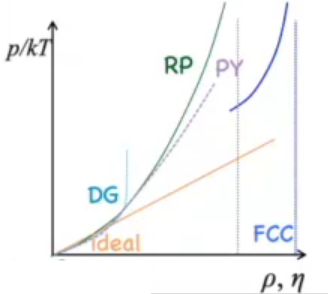
\includegraphics[width=0.3\textwidth]{figures/Confronto-chiusure.png}
	\caption{Confronto tra le varie chiusure.}
	\label{fig:chiusure-confronto}
\end{figure}
L'approssimazione RP non è molto buona per le sfere dure, tuttavia la si cita perché è utile nel caso Coulombiano.\\
Tramite simulazioni al computer è possibile anche connettere la fase completamente cristallina a quella disordinata, il risultato che si ottiene è il seguente:
\begin{figure}[H]
	\centering
	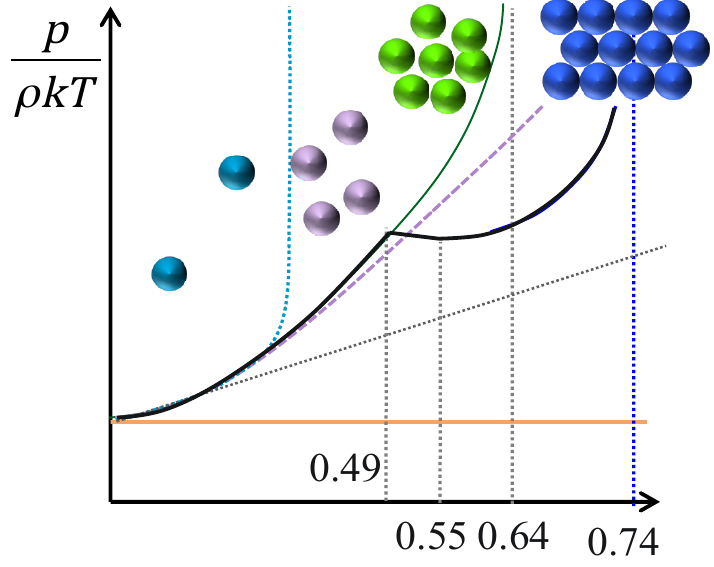
\includegraphics[width=0.5\textwidth]{figures/connessione-RP-PY-BG.png}
	\caption{Connessione tra le varie chiusure per formare un unico andamento.}
	\label{fig:PY-RP-BG}
\end{figure}
\subsection{Modello di Lennard Jones per le sfere}
\label{subsec:Modello di Lennard Jones per le sfere}
Il modello di lennard Jones differisce da quello a sfere dure per il fatto che contiene una buca di potenziale di profondità $\mathcal{E}$.
\begin{figure}[ht]
	\centering
	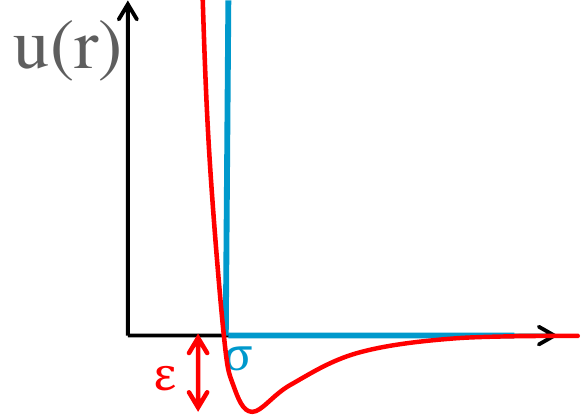
\includegraphics[width=0.3\textwidth]{figures/buca-Lennard-Jones.png}
	\caption{Confronto tra sfere dure e buca di Lennard Jones.}
	\label{fig:figures-buca-Lennard-Jones-png}
\end{figure}
Quindi se prima le grandezze scalavano spazialmente come $\sigma$ adesso (oltre a questa spaziatura) abbiamo anche una scala energetica: $\mathcal{E}/kT$ \footnote{Questo significa che un sistema alla temperatura $T$ ed energia $\mathcal{E}$ si comporta come un sistema a temperatura $2T$ ed energia $2\mathcal{E}$.}.\\
Possiamo vedere l'introduzione della interazione come una perturbazione del modello a sfere dure, per far questo possiamo considerare un ragionamento euristico: 
la pressione quando aggiungo l'interazione al modello delle sfere rigide deve diminuire, questo per via della maggiore attrazione presente tra le particelle:
\[
	P = P_\text{HS} - \ldots
.\] 
Questo effetto di diminuzione della pressione sarà tanto maggiore quanto più la densità è alta: 
\[
	P=P_\text{HS} - f(\rho )
.\] 
Essendo questo un effetto di correlazione a due corpi la dipendenza dalla densità della correzione non sarà lineare bensì quadratica, otteniamo quindi:
\[\begin{aligned}
	P
	=&
	P_\text{HS} - a \rho ^2 =\\
	=&
	\frac{\rho kT}{1-4\eta}-a\rho ^2=\\
	=&\frac{\rho kT}{1-b\rho }-a\rho ^2
.\end{aligned}\]
Utilizzando l'equazione di stato 
\[
	P 
	=
	\rho kT - \frac{\rho ^2}{6}\int r \frac{\partial u(r)}{\partial r} g(r) dr
.\]
Possiamo calcolare il valore di $a$, per approfondire aprire il March Tosy, a noi basta citare le linee guida per il calcolo e ci fidiamo:
\begin{itemize}
	\item Assumiamo che la parte dell'integrale divergente $r<\sigma$ sia già inclusa
		in $P_\text{HS}$, possiamo calcolare l'integrale direttamente per 
		$r>\sigma$ e porlo a questo punto uguale a $a\rho ^2$. Inoltre è
		necessario porre la risalita del potenziale avente un andamento del tipo
		$r^6$.
	\item Facciamo l'approssimazione di PY ponendo $g(r)\sim 1$ nell'integrale 
		rendendolo risolvibile, questo metodo ci fornisce l'equazione di stato 
		dei gas di Wan Der Waals.
\end{itemize}
Con questo metodo si conclude che:
\[
	\frac{P}{\rho kT} 
	=
	\frac{1}{1- \frac{2}{3}\pi\sigma^3\rho }
	-
\underbrace{
	\frac{16\pi}{9}\frac{\mathcal{E}}{kT}\sigma^3
}_{a/kT}	
	\rho 
.\] 
Abbiamo una equazione di stato per fluidi di Lennard Jones sempre nella approssimazione di fluido diluito. È importante notare la dipendenza del parametro $a$ dal valore di $\mathcal{E} /kT$, questo fa si che si ottengano curve sensibilmente differenti nel grafico di $P/kT$ come si mostra in Figura \ref{fig:-figures-Wan-Der-Waals-curve-dipendenza-ekT-png}.
\begin{figure}[ht]
	\centering
	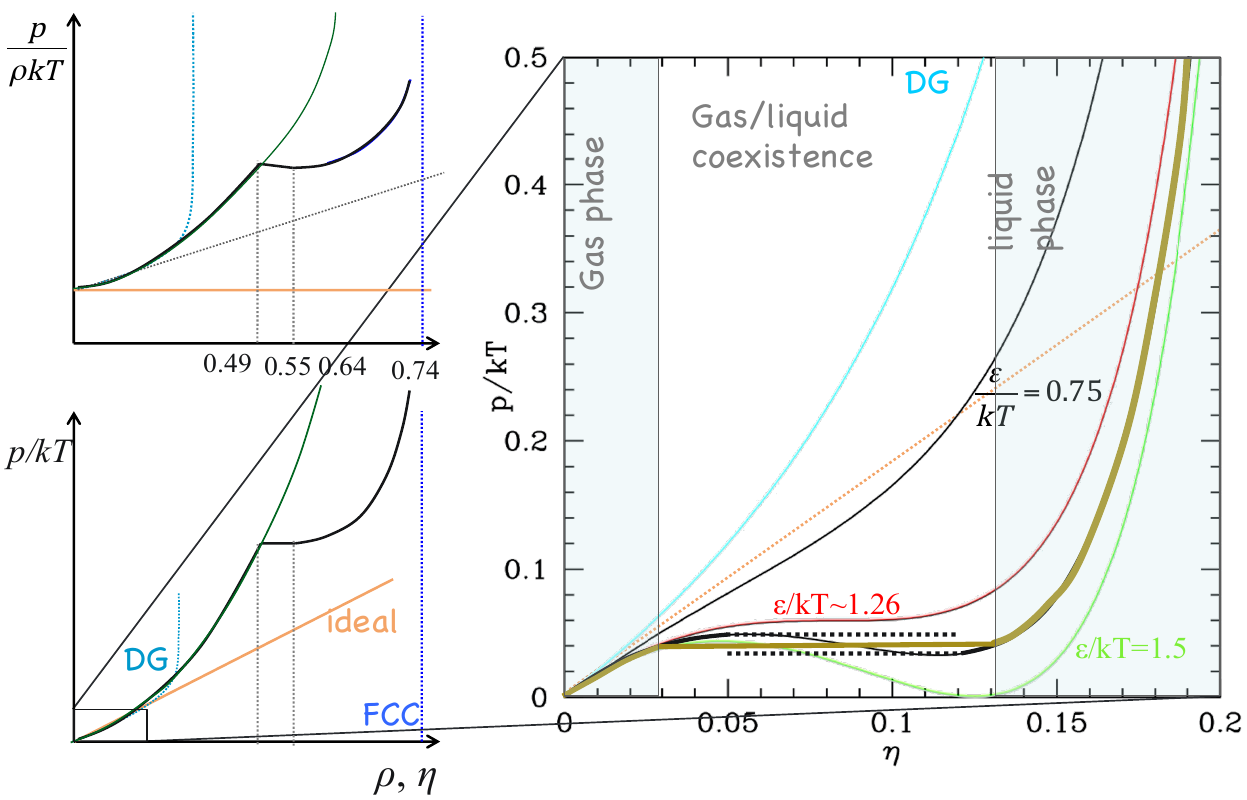
\includegraphics[width=0.6\textwidth]{figures/Wan-Der-Waals-curve--dipendenza-ekT.png}
	\caption{\scriptsize Curve nel grafico $P/kT$ per un fluido di Lennard Jones,
	questo modello funziona bene nella parte di grafico in basso a sinistra 
	evidenziata e zoommata con un rettangolo. È inoltre chiaro come si modifica quella
	zona di curva al variare del parametro $\mathcal{E} /kT$. La linea DG corrisponde 
	alle sfere dure (oppure a $a=0$).}
	\label{fig:-figures-Wan-Der-Waals-curve-dipendenza-ekT-png}
\end{figure}
Dalle curve in questa figura possiamo notare che all'aumentare del parametro $\mathcal{E} /kT$ si forma un flesso, concentriamoci su questa importante particolarità. \\
\begin{figure}[ht]
    \centering
    \incfig{cambio-statoWDV}
    \caption{Flesso nella curva per l'equazione di stato.}
    \label{fig:cambio-statoWDV}
\end{figure}
\noindent
Come possiamo notare dalla Figura \ref{fig:cambio-statoWDV} se ci spostiamo dall'origine verso la curva incontriamo un massimo nella pressione, viceversa spostandoci dall'altra parte otterremo un minimo nella pressione con successiva risalita. \\
Questa anomalia corrisponde ad un passaggio di fase: la pressione è discontinua alla densità. Precisamente questo rappresenta un passaggio di fase tra gas e liquido.
\newpage
\begin{fact}[Fasi nei vari modelli]{fact:Fasi nei vari modelli}
	Il modello di gas ideale permette soltanto una fase gassosa, il modello a sfere
	rigide permette di predire soltanto la separazione tra fase gassosa e fase solida,
	il modello di Lennard Jones permette di predire fase gassosa, fase liquida 
	e fase solida.
\end{fact}
Notiamo che è possibile anche continuare a seguire la curva tratteggiata senza fare il salto in un punto esatto, questo corrisponde alla situazione di liquido riscaldato (viceversa di gas raffreddato)
\footnote{Questo è ciò che si osserva facendo bollire l'acqua: capita che si superi la temperatura di fusione senza che effettivamente tale fusione avvenga. Questa è una situazione metastabile che viene rotta dalla aggiunta del sale.}.\\
Possiamo anche dire che tale flesso corrisponde al punto critico nel grafico $PT$.
\begin{figure}[ht]
	\centering
	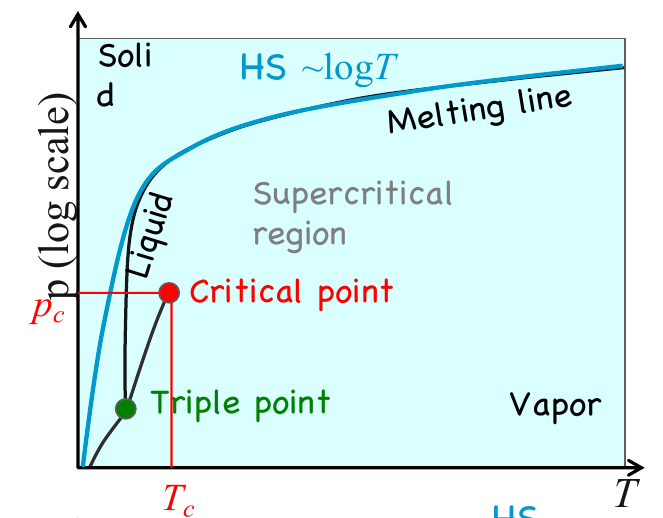
\includegraphics[width=0.4\textwidth]{figures/Punto-triplo.png}
	\caption{Punto critico nella curva $PT$.}
	\label{fig:figures-Punto-triplo-png}
\end{figure}
Quando l'energia $\mathcal{E}\to 0$ abbiamo che il punto critico viene mandato verso l'origine schiacciando anche il punto triplo verso questa direzione.\\
È interessante notare come nel grafico $T\rho $ invece "espandere" il potenziale delle sfere rigide nell'idea di Lennard Jones corrisponde ad "ampliare il campo visivo come si evince in Figura \ref{fig:figures-grafico-T-rho-png}.
\begin{figure}[ht]
	\centering
	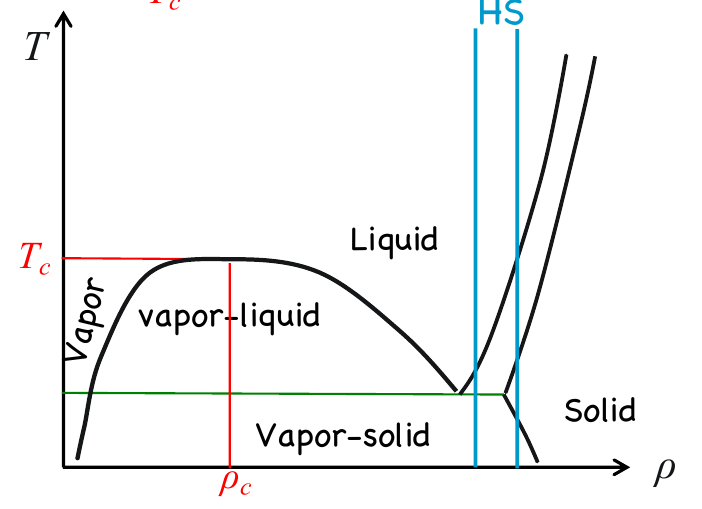
\includegraphics[width=0.4\textwidth]{figures/grafico-T-rho.png}
	\caption{\scriptsize Andamento $T-\rho $ per fluido di Lennard Jones a confronto con porzione di grafico vista dal modello Hard Sphere.}
	\label{fig:figures-grafico-T-rho-png}
\end{figure}
\subsection{Riscalamento di $S(q)$ e $g(r)$.}
\label{subsec:Riscalamento di $S(q)$ e $g(r)$.}
Abbiamo visto che i grafici di $S(q)$ e $g(r)$ tendono a sovrapporsi nella regione al di sopra del punto critico (spostandosi nel grafico $PT$) come in Figura \ref{fig:figures-grafici-shiftati-png}.\\
\begin{figure}[ht]
	\centering
	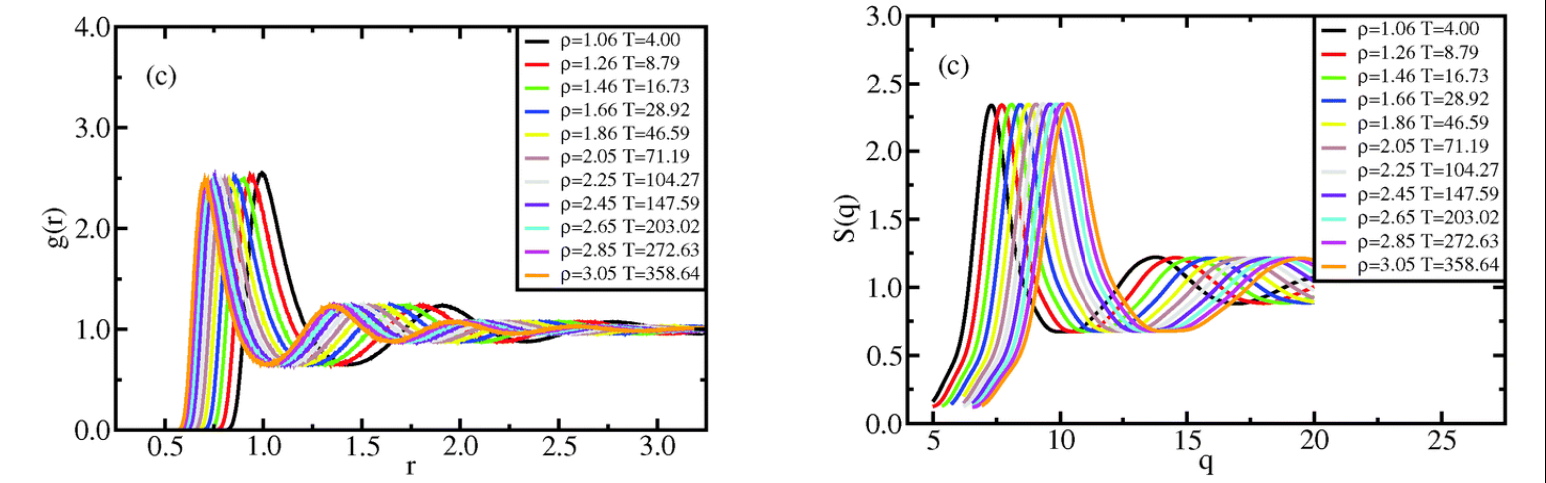
\includegraphics[width=0.9\textwidth]{figures/grafici-shiftati.png}
	\caption{Andamenti di $S(q)$ e $g(r)$.}
	\label{fig:figures-grafici-shiftati-png}
\end{figure}
Se normalizziamo la distanza $r\to r/\sigma$ (che equivale a fare $r\to r/\rho^{1/3}$) ed il potenziale $u\to u/kT$ allora otteniamo che tali curve si sovrappongono come possiamo vedere in Figura \ref{fig:reduced-Sg}.
\begin{figure}[ht]
	\centering
	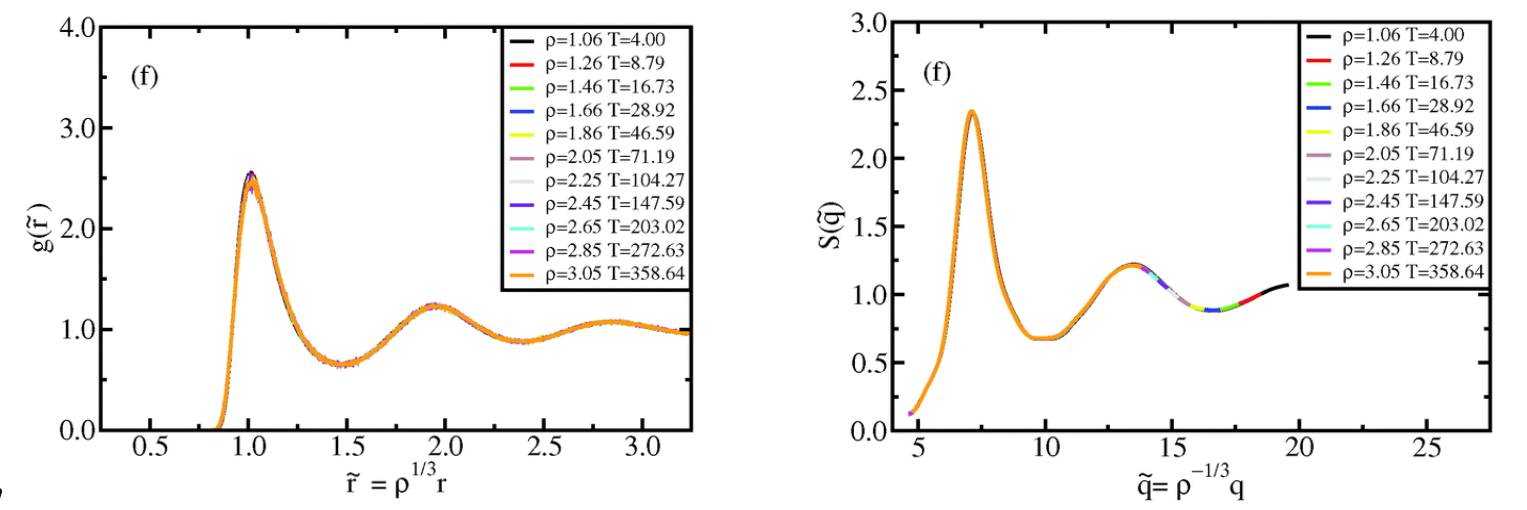
\includegraphics[width=0.9\textwidth]{figures/grafici-sovrapposti.png}
	\caption{Andamento di $S(q)$ e $g(r)$ con le variabili ridotte.}
	\label{fig:reduced-Sg}
\end{figure}
\subsection{Riassunto di HG,HS,LJ.}
\label{subsec:Riassunto di HG,HS,LJ.}
Nel seguente grafico possiamo vedere un riassunto delle formule saliente affrontate nell'ultima lezione:
\begin{figure}[H]
	\centering
	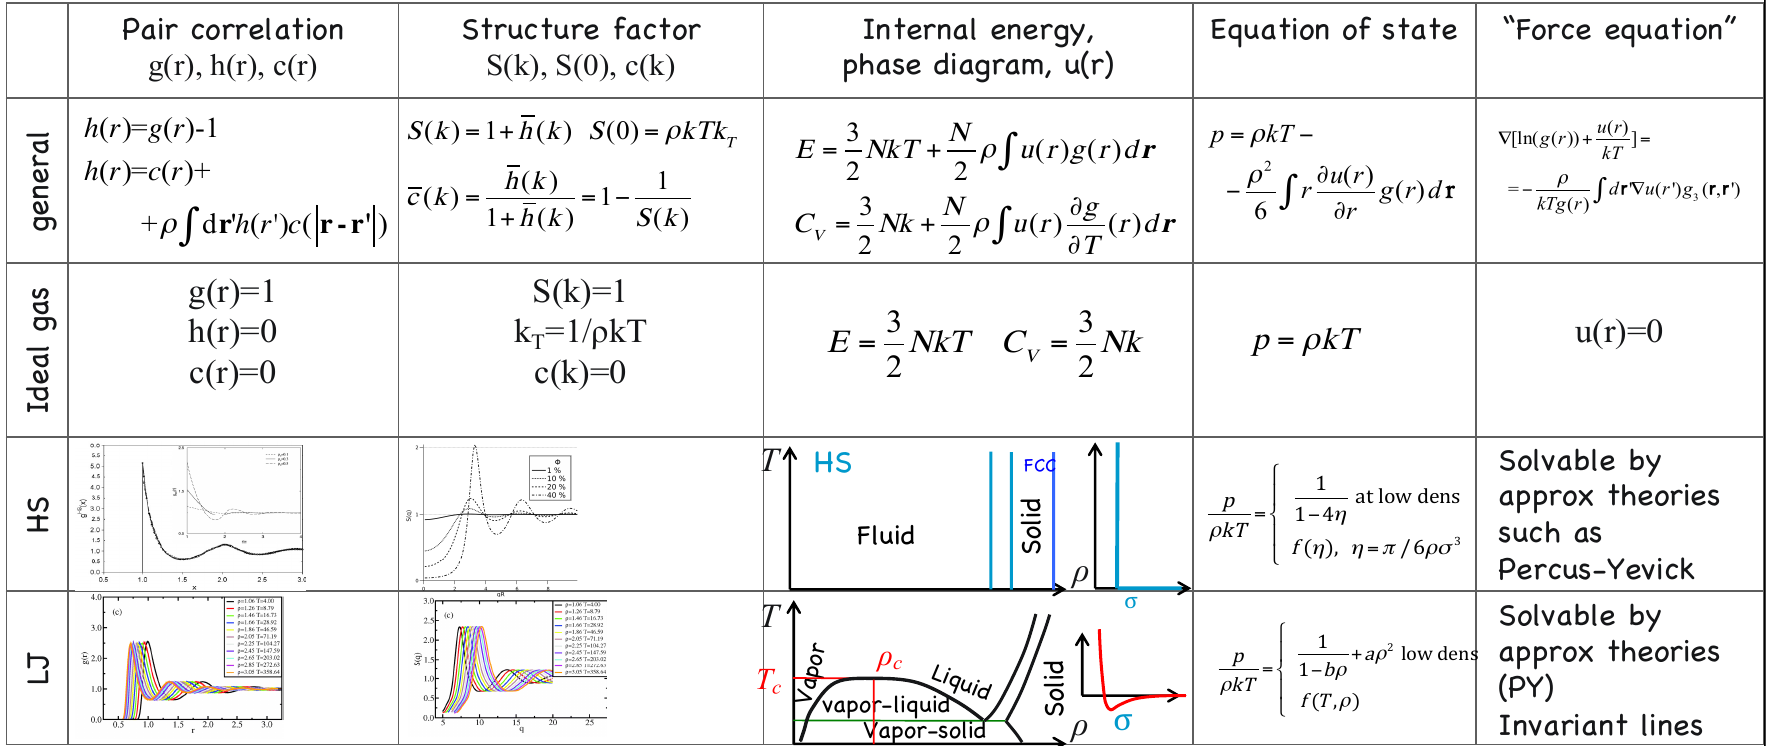
\includegraphics[width=1\textwidth]{figures/riassuntone-lez3-emezzo.png}
	\caption{Riassunto delle puntate precedenti.}
	\label{fig:figures-riassuntone-lez3-emezzo-png}
\end{figure}
\subsection{Fluidi quantistici: trattazione della condensazione di Bose.}
\label{subsec:Fluidi quantistici: trattazione della condensazione di Bose.}
Possiamo dire euristicamente che la regione di interesse quantistico nel grafico $PT$ sarà quella a basse temperature. \\
Normalmente si ha che un cristallo si rompe quando le fluttuazioni termiche diventano più grandi della distanza interatomica, tuttavia a basse temperature sono le fluttuazioni quantistiche diventano più grandi di quelle termiche, di conseguenza la temperatura assume un "ruolo minore" nelle transizioni di fase.\\
Questo ragionamento spiega in grandi linee la formazione di un nuovo stato della materia: il superfluido, la transizione di fase in questo stato non è guidata dalle fluttuazioni termiche ma dalle fluttuazioni quantistiche.
\begin{figure}[ht]
	\centering
	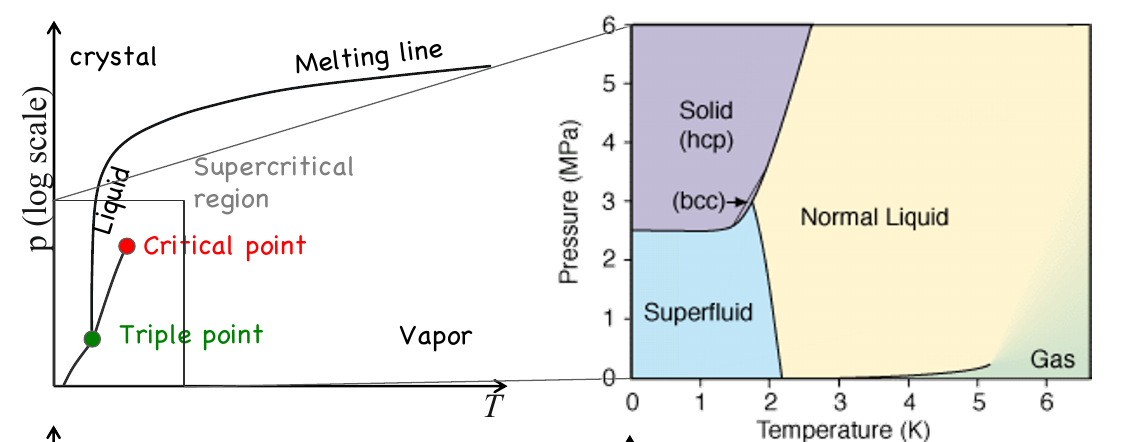
\includegraphics[width=0.7\textwidth]{figures/superfluido.png}
	\caption{Formazione del superfluido.}
	\label{fig:ffigures-superfluido-png}
\end{figure}
Per completezza si mostra anche come varia il grafico $T\rho $ nel caso quantistico (diventa molto complicato).
\begin{figure}[ht]
	\centering
	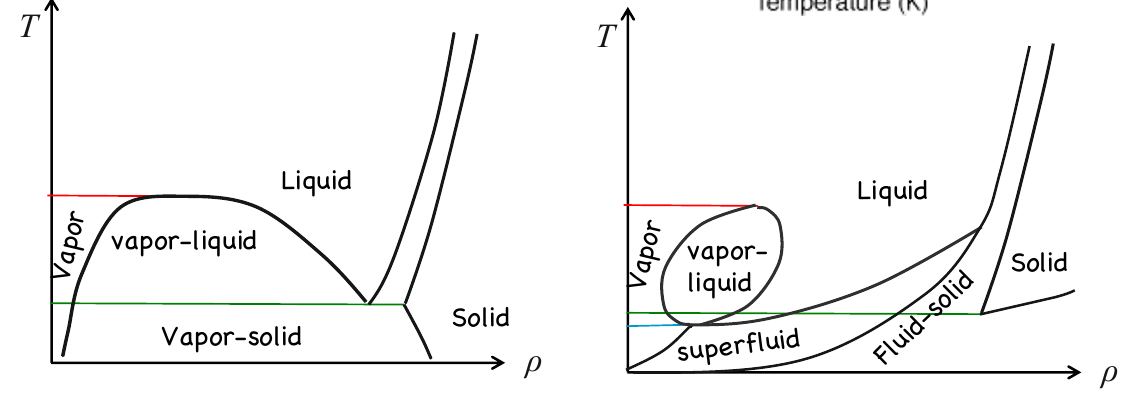
\includegraphics[width=0.7\textwidth]{figures/Tr-quantistico.png}
	\caption{Andamento del grafico $T\rho $ nel caso classico e nel caso quantistico.}
	\label{fig:figures-Tr-quantistico-png}
\end{figure}
\subsection{Colloidi.}
\label{subsec:Colloidi.}
Il potenziale di Lennard Jones si applica bene nel caso di "piccole particelle che corrispondono ai gas nobili", oppure in generale per atomi in cui il dipolo permanente è piccolo o assente.
\begin{fact}[Applicabilità di Lennard Jones]{fact:Applicabilità di Lennard Jones}
	Il potenziale di Lennard Jones è applicabile nel caso di sistemi composti da
	particelle neutre non polarizzate.
\end{fact}
Un ottimo caso in cui è possibile applicare il potenziale di Lennard Jones è quello riguardante le particelle colloidali \footnote{Particelle disperse in un'altra sostanza in cui sono libere di muoversi.}.
Un esempio di colloide sono le proteine globulari.\\
Per poter utilizzare un modello alla Lennard Jones in questo caso particolare è necessario (essendo le particelle in genere molto più grandi della scala atomica \footnote{Quindi $\sigma$ molto più grande di quelli utilizzati fin'ora.}) utilizzare una forma di potenziale avente un range di interazione stretto senza diminuire $\mathcal{E}$. Potrebbe essere utile avere un altro parametro che regola la larghezza del potenziale.\\
Applicare queste modifiche cambia nuovamente il diagramma di fase come in Figura \ref{fig:figures-colloidi-png}.\\
\begin{figure}[ht]
	\centering
	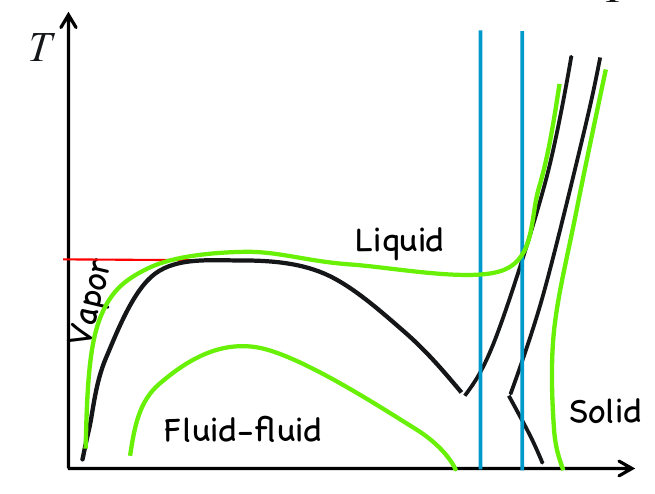
\includegraphics[width=0.3\textwidth]{figures/colloidi.png}
	\caption{Modifiche al grafico della equazione di stato per i collodi.}
	\label{fig:figures-colloidi-png}
\end{figure}
Quando il range di attrazione diventa sufficientemente piccolo perdiamo di nuovo la fase liquida. Questa fase infatti esiste stabilizzata se vi è un potenziale attrattivo sufficiente.\\
Dobbiamo comunque puntualizzare una caratteristica importante dei collodi, infatti questi sono immersi in una sostanza liquida. Dire quindi che questi sono in una fase gassosa è fuorviante, in realtà la fase gassosa per questi corrisponde ad una fase completamente dispersa nel fluido, una fase solida corrisponde invece ad un precipitato.\\
Possiamo immaginare invece una fase liquida come una fase in cui i colloidi sono tutti vicini tra loro a formare un oggetto "appiccicaticcio".
\subsection{Repulsione a lungo raggio: cristallo di Wiegner.}
\label{subsec:Repulsione a lungo raggio: cristallo di Wiegner.}
Consideriamo un caso estremo di potenziale di Coulomb puro: elettroni in un background inerte positivo (plasma).\\
Il potenziale è a lungo lungo raggio ma allo stesso tempo questi hanno $\sigma=0$ non essendoci una repulsione Hardcore.\\
Sappiamo che i fermioni non fanno condensazione per via della loro distribuzione quantistica, tuttavia a basse densità possono raggiungere una configurazione stabile detta cristallo di Wiegner. Questa configurazione può essere rotta aumentando la densità, in tal modo il cristallo si fonde.\\
Le oscillazioni che possono rompere il cristallo possono essere di natura quantistica se la temperatura supera $T\propto h^2 /m\rho ^{2/3}$ oppure quantistiche se l'energia delle fluttuazioni supera $k_F^2\sim\rho ^{2/3}$.\\
La cristallizzazione di Wiegner si forma quando si raggiunge un equilibrio tra energia cinetica degli elettroni e l'energia di scambio, questo avviene quando la distanza tra un elettrone ed un altro è dell'ordine delle 100 u.a. ($\rho \sim 10^{18}$ el/cm$^3$) \footnote{Consideriamo che la densità di un normale fluido quando arriva a cristallizzare è $\sim 10^{24}$ cm$^3$.}.
Si ha quindi che la cristallizzazione di Wiegner avviene e basse densità ed a basse temperature.
\begin{figure}[ht]
	\centering
	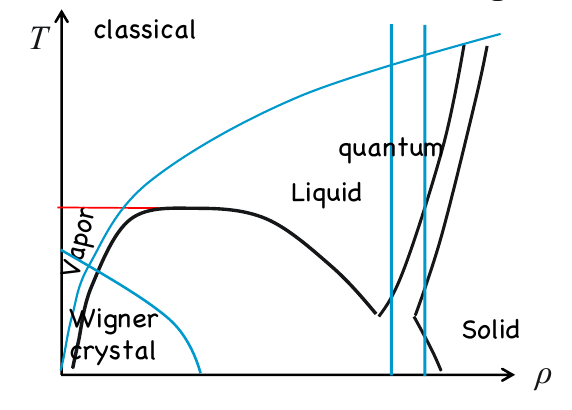
\includegraphics[width=0.4\textwidth]{figures/cristallo-Wiegner.png}
	\caption{Zona di cristallizzazione di Wiegner confrontata con le altre viste fino ad ora.}
	\label{fig:figures-cristallo-Wiegner-png}
\end{figure}
\subsection{Interazioni a lungo raggio ed approssimazione di Random Phase.}
\label{subsec:Interazioni a lungo raggio.}
Tornando nel regime classico quando siamo in presenza di un potenziale Coulombiano le approssimazioni fatte in precedenza ($g(r)\sim 1$, $u(r)\sim 0$) smettono di funzionare, questo perché funzionavano soltanto a grandi distanze (alternativamente dovevano esistere soli interazioni a corto range).\\
È necessario tornare alla formula iniziale in cui abbiamo utilizzato l'approssimazione di Born Green (o di sovrapposizione):
\[\begin{aligned}
	\nabla_{\v{r}_1}g(\left| \v{r}_1-\v{r}_2 \right| )
	=&
	-\frac{g(\left| \v{r}_1-\v{r}_2 \right|)}{kT}
	\nabla_{\v{r}_1}u(\left| \v{r}_1-\v{r}_2 \right| )+\\
	 &- \frac{\rho }{kT}\int d\v{r}_3\nabla_{\v{r}_1}u(\left| \v{r}_1-\v{r}_3\right| )
	g(\left| \v{r}_1-\v{r}_2 \right| )
	g(\left| \v{r}_2-\v{r}_3 \right| )
	g(\left| \v{r}_1-\v{r}_3 \right| )
.\end{aligned}\]
Non potendo considerare $g(r)$ unitario e necessario ricordare come era legato con $S(q)$ e la funzione $\rho $, conviene quindi andare nello spazio di Fourier e considerare delle funzioni globali:
\[
	\rho g(r)=\frac{1}{N}\left<\sum_{i\neq j}^{} \delta(r-(r_i-r_j)) \right>
	\xrightarrow{FT}
	S(k)= \frac{1}{N}\left< \overline{\rho }(k)\overline{\rho}(-k) \right>
.\] 
In cui $\overline{\rho }$ è la fluttuazione della densità locale. Per tali fluttuazioni si ha:
\[
	\overline{\rho } = FT \left[ \sum_{i}^{} \delta(\v{r}-\v{r}_i) \right]
	= \sum_{i}^{} e^{i\v{k}\cdot\v{r}_i}
.\] 
Combinando le 3 ultime equazioni si ottiene che:
\[
	S(k)
	=
	1+\frac{1}{Nk^2}\sum_{k'}^{} \frac{\overline{u}(k')}{kT}
	\left<\overline{\rho }(k)\overline{\rho }(k')
	\overline{\rho }(k+k') \right>
	\v{k}\cdot\v{k}'
.\] 
L'approssimazione di Random Phase assume un interferenza distruttiva tra i termini aventi $k$ differenti all'interno delle 3 $\rho $ \footnote{Quindi deve essere $k\neq k'\neq k+k'$.}, quindi sopravvive soltanto un termine avente $k'=-k$. Si ottiene allora:
\[
	S(k) = \frac{1}{1+\rho \overline{u}(k)/kT}
.\] 
Quindi possiamo ricavare anche $c(r)$ viste le sue relazioni in trasformata con $S(k)$:
\[
	\overline{c}(k) =- \frac{\rho \overline{u}(k)}{kT} 
	\implies 
	c(r) = - \frac{u(r)}{kT}
.\] 
Questo è lo stesso risultato ottenuto con l'approssimazione di Abe nel limite asintotico, la differenza sta nel fatto che con la RP la si usa in tutto lo spazio.\\
Possiamo vedere la qualità di questa approssimazione confrontandola con alcuni dati sperimentali sulla  $g(r)$:
\begin{figure}[ht]
	\centering
	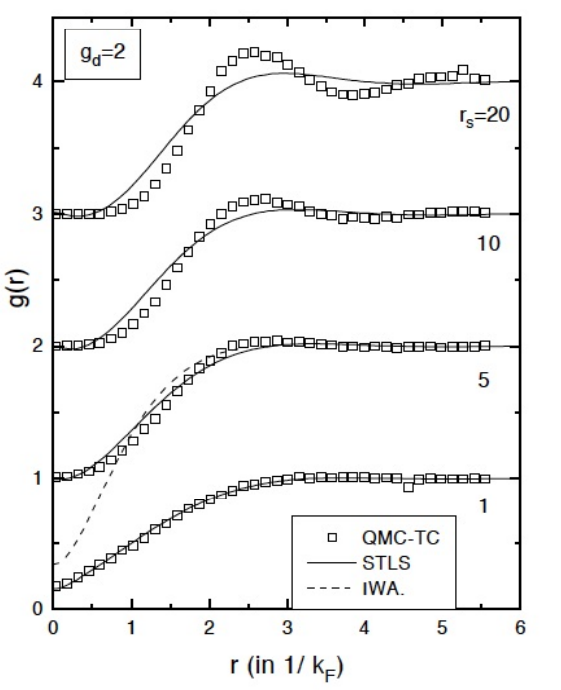
\includegraphics[width=0.3\textwidth]{figures/RP-coulomb.png}
	\caption{Approssimazione di Random Phase per un fluido Coulombiano.}
	\label{fig:figures-RP-coulomb-png}
\end{figure}
\subsection{Cosa devo sapere all'esame?}
\label{subsec:Cosa devo sapere all'esame?}
\begin{itemize}
	\item L'approssimazione PY funziona molto bene per i potenziali Hardcore.
	\item Per i fluidi LJ il potenziale PY funziona bene in media con eccezione
		in presenza di picchi.
	\item HNC (Abe) funziona bene per sfere soffici.
	\item RPA non è utilizzata generalmente per liquidi Hardcore. É invece utilizzata 
		per i liquidi Coulombiani in cui abbiamo interazioni a lungo raggio.
\end{itemize}
